\subsection{Leverage, influence, \emph{and} precision}

\begin{figure}[htb!]
  \centering
  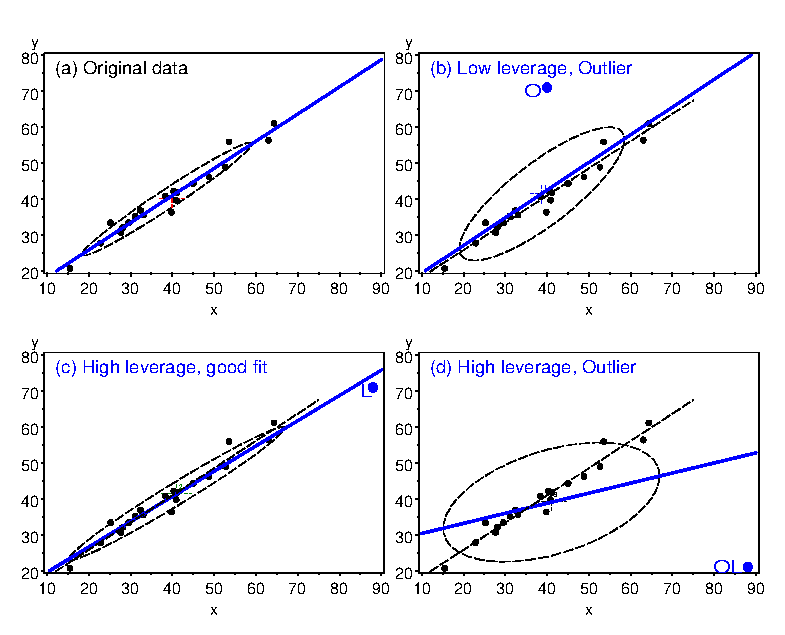
\includegraphics[width=\textwidth,clip]{fig/levdemo21}
  \caption{Leverage-Influence quartet with data ellipses. (a) Original data;
  (b) Adding one low-leverage outlier (O); (c) Adding one ``good'' leverage point (L);
  (d) Adding one ``bad'' leverage point (OL).
  In panels (b)--(d) the dashed black line is the fitted line for the original
  data, while the thick solid blue line reflects the  regression including the additional point.
  The data ellipses show the effect of the additional point on precision.}%
  \label{fig:levdemo21}
\end{figure}

The topic of leverage and influence in regression is often introduced with graphs
similar to \figref{fig:levdemo21}, what we call
the ``leverage-influence quartet.''
In these graphs, a bivariate sample of $n=20$ points was first generated
with $x \sim \mathcal{N}(40, 10)$ and $y \sim10 +  0.75 x + \mathcal{N}(0, 2.5)$.
Then, in each of
panels (b)--(d) a single point is added at the locations shown, to represent, respectively,
a low-leverage point with a large residual,\footnote{In this context, a residual is ``large'' when the point in question deviates substantially from the regression line for the rest of the data---what is sometimes termed a ``deleted residual'': see below.} a high-leverage point with small residual
(a ``good'' leverage point), and a high-leverage point with large residual
(a ``bad'' leverage point).  The goal is to visualize how leverage ($\propto (x-\bar{x})^2$) and
residual ($y - \hat{y}^{*}$) (where $\hat{y}^{*}_{i}$ is the fitted value for observation $i$, computed on the basis of an auxiliary regression in which observation $i$ is deleted) combine to produce influential points---those that affect
the estimates of $\vec{\beta} = (\beta_0 , \beta_1)\trans$.


The ``standard'' version of this graph shows \emph{only} the fitted regression lines for each
panel. So, for the moment, ignore the data ellipses in the plots.
The canonical, first-moment-only, story behind the standard version is that the points added in panels
(b) and (c) are not harmful---the fitted line does not change very much when these
additional points are included. Only the bad leverage point, ``OL,'' in panel (d) is harmful.

\begin{figure}[htb!]
  \centering
  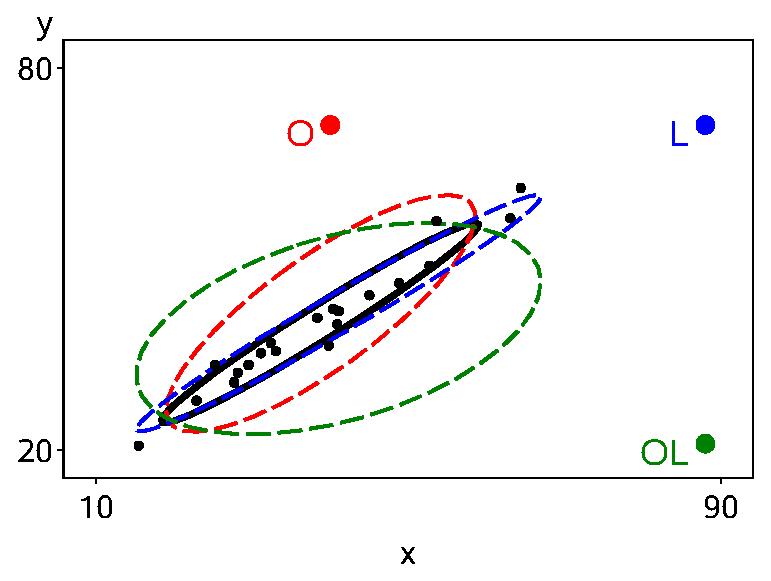
\includegraphics[width=.5\textwidth,clip]{fig/levdemo22}
  \caption{Data ellipses in the Leverage-Influence quartet. This graph overlays the data ellipses
  and additional points from the four panels of \figref{fig:levdemo21}. It can be seen that only the
  OL point affects the slope, while the O and L points affect precision of the estimates in opposite
  directions.}%
  \label{fig:levdemo22}
\end{figure}

Adding the data ellipses to each panel immediately makes it clear that there is a second-moment
part to the the story---the effect of unusual points on the \emph{precision} of our estimates
of $\vec{\beta}$.  Now,
we see \emph{directly} that there is a big difference in impact between
the low-leverage outlier (panel (b)) and the high-leverage, small-residual case (panel (c)),
even though their effect on coefficient estimates is negligible.
In panel (b), the single outlier inflates the estimate of residual variance (the size of the
vertical slice of the data ellipse at $\bar{x}$).

To make the added value of the data ellipse more apparent, we overlay the data ellipses from
\figref{fig:levdemo21} in a single graph, shown in
\figref{fig:levdemo22}, to allow direct comparison.  Because you now know that regression lines
can be visually estimated as the locus of vertical tangents, we suppress these lines in the
plot to focus on precision.  Here, we can also see why the high-leverage
point ``L'' (added in panel (c) of \figref{fig:levdemo21}) is called a ``good leverage point.''
By increasing the standard deviation of $x$, it makes the data ellipse somewhat more elongated,
giving increased precision of our estimates of $\vec{\beta}$. Whether a ``good'' leverage point is \emph{really} good depends upon our faith in the regression model (and in the point), and may be regarded either as increasing the precision of $\hat{\vec{\beta}}$ or providing an illusion of precision.

